
% Colorer un graphe
La coloration d'une carte de pays consiste à attribuer une couleur à chacun des pays de manière à ce que deux pays voisins soient de couleurs différentes.
Étudier ces techniques de coloration revient de façon plus abstraite à travailler sur des graphes.
Le champ d'applications de la coloration de graphes est très vaste et couvre des domaines aussi variés que le problème de l'attribution de fréquences dans les télécommunications, la conception de puces électroniques ou l'allocation de registres en compilation.
Soulignons que tous les graphes considérés dans ce sujet sont non-orientés. Quelques rappels de syntaxe Python figurent dans l'annexe \ref{2024_CCINP_TSI_Info_ann_02}.

\section{Des algorithmes pour colorer un graphe \label{2024_CCINP_TSI_Info_sec_01}}
\subsection{Introduction sur un exemple \label{2024_CCINP_TSI_Info_sec_01_1}}
On cherche à colorer une carte de pays avec comme seule contrainte que deux pays ayant une frontière commune ne peuvent être de la même couleur.
Comme les pays, les couleurs sont numérotées à partir de zéro.
À titre d'exemple, on considérera la carte suivante (figure \ref{2024_CCINP_TSI_Info_fig_01}), comportant 8 pays numérotés de 0 à 7, que l'on représentera par le graphe $\indice{G}{ex}$, donné en figure \ref{2024_CCINP_TSI_Info_fig_02}.

\begin{figure}[!h]
\centering
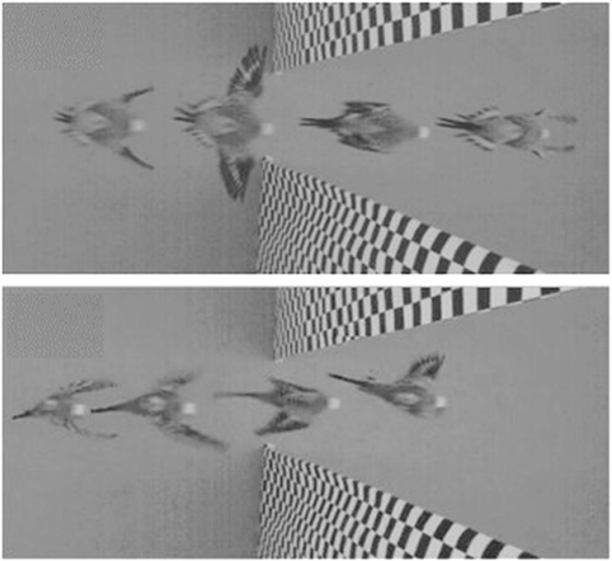
\includegraphics[width=.6\linewidth]{fig_01}
\caption{Exemple d'une carte de pays \label{2024_CCINP_TSI_Info_fig_01}}
\end{figure}

\begin{figure}[!h]
\centering
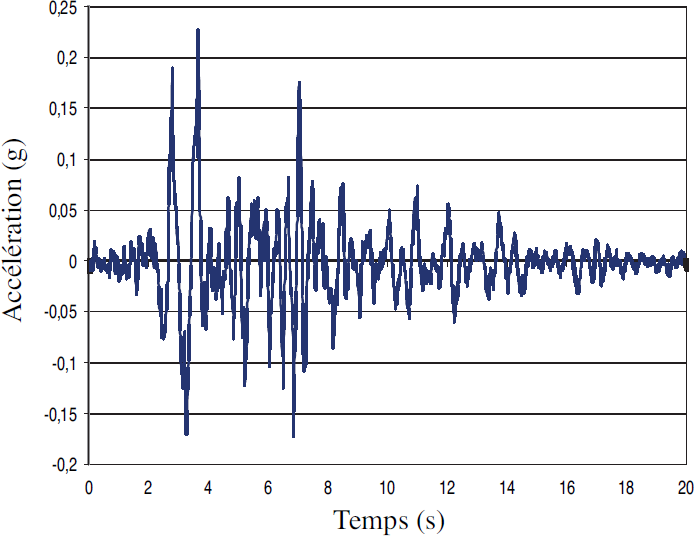
\includegraphics[width=.6\linewidth]{fig_02}
\caption{Graphe $\indice{G}{ex}$ associé à la carte de pays de la figure \ref{2024_CCINP_TSI_Info_fig_01}\label{2024_CCINP_TSI_Info_fig_02}}
\end{figure}

Ainsi, sur le graphe de la figure \ref{2024_CCINP_TSI_Info_fig_02}, deux pays sont voisins si et seulement si les sommets correspondants sont reliés par une arête.


% Q01
%\question{Un graphe peut être représenté par une matrice d'adjacence.
%Le DR*** contient la matrice d'adjacence pré-remplie du graphe $\indice{G}{ex}$. La compléter et expliquer le processus de construction.}
\question{Un graphe peut être représenté par une matrice d'adjacence.
Donner la matrice d'adjacence associée au graphe $\indice{G}{ex}$ et expliquer le processus de construction.}

\ifprof
\begin{corrige}
Pour remplir la matrice d'adjacence, si deux sommets $i$ et $j$ sont voisins alors $\indice{G}{ex}[i][j] = 1$.
 Sinon,  $\indice{G}{ex}[i][j] = 0$. 
$\indice{G}{ex}=
\begin{pmatrix}
%0 	& 1	& 2	& 3	& 4	& 5	& 6	& 7	\\ 
0 	& 1	& 0	& 1	& 1	& 0	& 1	& 1	\\ 
1 	& 0	& 1	& 1	& 0	& 0	& 0	& 0	\\ 
0 	& 1	& 0	& 1	& 0	& 0	& 0	& 0	\\ 
1	& 1	& 1	& 0	& 1	& 0	& 0	& 0	\\ 
1 	& 0	& 0	& 1	& 0	& 1	& 1	& 1	\\ 
0 	& 0	& 0	& 0	& 1	& 0	& 1	& 1	\\ 
1 	& 0	& 0	& 0	& 1	& 1	& 0	& 1	\\ 
1 	& 0	& 0	& 0	& 1	& 1	& 1	& 0	\\ 
\end{pmatrix}$

On a aussi : 
\lstinputlisting[firstline=2,lastline=9]{CCINP_TSI_Informatique.py}
\end{corrige}
\else
\fi

Une autre manière de représenter en mémoire un graphe est d'utiliser une liste d'adjacence. La liste d'adjacence d'un graphe (constitué de sommets numérotés de 0 à $n-1$) est une liste \lstinline{LA}, telle que \lstinline{LA[i]} est la liste des sommets voisins du sommet \lstinline{i}. Par convention, les voisins énumérés dans \lstinline{LA[i]} seront listés dans l'ordre croissant.

% Q02
\question{Donner la liste d'adjacence du graphe  $\indice{G}{ex}$ présenté en exemple.}
\ifprof
\begin{corrige}
On a  :

%\lstinline{LA = [[1,3,4,6,6],[0,2,3],[1,3],[0,1,2,4],[0,3,5,6,7],[4,6,7],[0,4,5,7],[0,4,5,6]]}.

\lstinputlisting[firstline=12,lastline=12]{CCINP_TSI_Informatique.py}

\end{corrige}
\else
\fi

% Q03
\question{Donner un avantage et un inconvénient d'une représentation par matrice d'adjacence. Donner un avantage et un inconvénient d'une représentation par liste d'adjacence.}
\ifprof
\begin{corrige}
\textbf{Matrice d'adjacence :}
\begin{itemize}
\item [$+$] Le test d’adjacence de deux sommets se fait en temps constant.
\item [$+$] Rajouter ou supprimer une arête (ou un arc) peut se faire en temps constant.
\item [$-$] Ajouter ou supprimer un sommet nécessite un temps proportionnel à $n^2$.
\item [$-$] Pour récupérer les voisins/successeurs d’un nœud, il faut parcourir toute la ligne de la matrice :
l’opération se fait donc en $\mathcal{O}(n)$, ce qui est regrettable si le degré sortant du noeud est petit devant $n$.
\item [$-$] On consomme une mémoire proportionnelle à $|V|^2$, même quand la taille du graphe est de l’ordre de $n$ (graphe creux).
\end{itemize}


\textbf{Liste d'adjacence :}
\begin{itemize}
\item [$+$] La mémoire utilisée est de l’ordre de $|E| + |V|$, ce qui est nettement mieux que $|V|^2$ si le graphe est
creux.
\item [$+$] On a directement accès à la liste des voisins d’un noeud : la parcourir prend un temps proportionnel
au degré sortant du noeud.% (et pas à $|V|$).
\item [$+$] Ajouter un noeud peut normalement se faire en temps $|V|$ (si l’ajout n’impose pas de renuméroter
les noeuds déjà présents).
%\item  Si l’on a besoin d’un accès en temps raisonnable aux prédécesseurs d’un noeud (dans le cas orienté),
%il faut stocker séparément le tableau de listes correspondant.
\item [$-$]  Le test d’adjacence ne se fait plus en temps constant (mais en temps proportionnel au degré du
nœud).
\item [$-$] Si le graphe est dense, on consommera plus de mémoire (d’un facteur constant) qu’avec une matrice d’adjacence.
\item [$-$] Ajouter ou supprimer une arête n’est pas aussi évident que dans une matrice d’adjacence : suivant
l’opération précise que l’on souhaite faire, la complexité peut être unitaire ou proportionnelle aux
degrés des nœuds impactés.
\item [$-$] Supprimer un noeud n’est pas pratique : le plus simple est de reconstruire entièrement le graphe (en
un temps $\mathcal{O}\left(|E| + |V|\right)$).
\end{itemize}

\end{corrige}
\else
\fi

On rappelle que le degré d'un sommet $s$ d'un graphe $G$ est le nombre de voisins du sommet $s$, c'est-à-dire le nombre de sommets reliés à $s$.

% Q04
%\question{Le DR*** fournit le tableau des degrés des différents sommets du graphe $\indice{G}{ex}$. Le compléter.}
\question{Compléter le tableau des degrés des différents sommets du graphe $\indice{G}{ex}$ est donné ci-dessus.}
\ifprof
\begin{corrige}
\begin{center}
\begin{tabular}{lcccccccc}
\hline
\textbf{Sommet} 	& 0 & 1 & 2 & 3 & 4 & 5 & 6 & 7 \\
\hline
\textbf{Degré} 		& 5 & 3 & 2 & 4 & 5 & 3 & 4 & 4\\
\hline
\end{tabular}
\end{center}

\end{corrige}
\else

\fi
\begin{center}
\begin{tabular}{lcccccccc}
\hline
\textbf{Sommet} 	& 0 & 1 & 2 & 3 & 4 & 5 & 6 & 7 \\
\hline
\textbf{Degré} 		& & & & & & & & \\
\hline
\end{tabular}
\end{center}


\subsection{Tester si une coloration est valide}

% Q05
\question{Écrire une fonction \lstinline{voisins} avec trois arguments, deux nombres entiers distincts \lstinline{i} et \lstinline{j} et une liste d'adjacence \lstinline{LA} représentant un graphe, qui renvoie \lstinline{True} si les sommets numérotés \lstinline{i} et \lstinline{j} sont reliés par une arête et \lstinline{False} sinon.}
\ifprof
\begin{corrige}~\\ \vspace{-.5cm}
\lstinputlisting[firstline=16,lastline=33]{CCINP_TSI_Informatique.py}
\end{corrige}
\else
\fi

On considère une carte de pays, représentée par un graphe \lstinline{G} pour laquelle on a une proposition de coloration donnée par une liste \lstinline{C}. Ainsi, \lstinline{C[i]} donne le numéro de la couleur attribuée au sommet \lstinline{i}. On souhaite déterminer si la coloration proposée est valide (deux sommets du graphe reliés par une arête ne peuvent pas être de la même couleur).

% Q06
\question{Écrire la fonction \lstinline{coloration_valide} avec pour arguments une liste d'adjacence \lstinline{LA} et une liste de couleurs \lstinline{C}, qui renvoie \lstinline{True} si la coloration est valide, \lstinline{False} sinon.}
\ifprof
\begin{corrige}~\\ \vspace{-.5cm}
\lstinputlisting[firstline=36,lastline=41]{CCINP_TSI_Informatique.py}
\end{corrige}
\else
\fi

% Q07
\question{\label{2024_CCINP_TSI_Info_q_07} Pour un graphe comportant \lstinline{n} sommets, quelle est la complexité temporelle dans le pire des cas de la fonction \lstinline{coloration_valide} ?}
\ifprof
\begin{corrige}
Dans le pire des cas, on a $n$ sommets tous interconnectés. Chaque sommet a donc $n-1$ voisins. 
En comptant le nombre de comparaisons, on a $C(n) = \sum\limits_{i=1}^{n}\sum\limits_{j=1}^{n} 1 = \mathcal{O}\left(n^2\right)$.
\end{corrige}
\else
\fi

\subsection{Un algorithme intuitif de coloration}

L'attribution des couleurs à chaque sommet est caractérisée par une liste \lstinline{C} où \lstinline{C[i]} est la couleur attribuée au sommet \lstinline{i}; \lstinline{C[i]} vaut $-1$ si la couleur n'est pas encore attribuée. La liste \lstinline{C} ne contient que des  $-1$ au départ et ses valeurs sont modifiées progressivement au fur et à mesure que les couleurs sont attribuées.


% Q08
\question{\label{2024_CCINP_TSI_Info_q_08} On suppose (dans cette question seulement) que \lstinline{n} est une constante déjà définie. Écrire la ou les instruction(s) permettant de créer une liste initiale \lstinline{C} composée de \lstinline{n} éléments valant $-1$.}
\ifprof
\begin{corrige}~\\ \vspace{-.5cm}
\lstinputlisting[firstline=46,lastline=50]{CCINP_TSI_Informatique.py}
\end{corrige}
\else
\fi



% Q09
\question{\label{2024_CCINP_TSI_Info_q_09} Compléter la fonction \lstinline{colore_sommet} ayant trois arguments, la liste \lstinline{C} des couleurs attribuées, le numéro \lstinline{s} du sommet à colorer et la liste d'adjacence \lstinline{LA} caractérisant le graphe. Cette fonction ne renvoie rien mais modifie la liste \lstinline{C} en donnant à \lstinline{C[s]} la plus petite couleur possible, en fonction des couleurs des sommets voisins qui sont déjà colorés. }

Par exemple, pour le graphe $\indice{G}{ex}$, prenons \lstinline{C = [0,1,-1,-1,-1,-1,-1,-1]}. Les sommets 0 et 1 ont donc déjà été colorés avec les couleurs \lstinline{C[0] = 0} et \lstinline{C[1] = 1}.

L'appel \lstinline{colore_sommet(C, 2, LA)} modifie la liste \lstinline{C} en \lstinline{C  = [0,1,0,-1,-1,-1,-1,-1]}. Cela veut dire que le sommet 2, adjacent au sommet 1 mais pas au sommet 0, a reçu la même couleur que le sommet 0.


\ifprof
\begin{corrige}
NDLR -- XP : Question pas si évidente. Il y a surement une solution plus simple.


\lstinputlisting[firstline=53,lastline=76]{CCINP_TSI_Informatique.py}
\end{corrige}

\else

\fi
\begin{lstlisting}
def colore_sommet(C,s,LA) :
    # on détermine la liste des couleurs des voisins de s déjà colorés
    coul_vois = []
    
    # coul_vois est maintenant déterminée et on recherche la
    # plus petite couleur, notée num_coul, absente de coul_vois:
    
    # la valeur num_coul trouvée devient la couleur du sommet s :
\end{lstlisting}
% Q10
\question{\label{2024_CCINP_TSI_Info_q_10} À l'aide de la question \ref{2024_CCINP_TSI_Info_q_09}, écrire une fonction \lstinline{colorer1} avec pour argument une liste \lstinline{LA} caractérisant un graphe, qui crée et renvoie la liste \lstinline{C} des numéros des couleurs attribuées en colorant les sommets un par un par ordre croissant de leurs numéros.}

Par exemple, l'application de la fonction \lstinline{colorer1} au graphe $\indice{G}{ex}$ renverra la liste de couleurs \lstinline{[0,1,0,2,1,0,2,3]}.
\ifprof
\begin{corrige}~\\ \vspace{-.5cm}
\lstinputlisting[firstline=80,lastline=84]{CCINP_TSI_Informatique.py}
\end{corrige}
\else
\fi


L'ordre de coloration imposé à la question précédente est arbitraire. On souhaite maintenant colorer le graphe en traitant les sommets selon un ordre arbitraire donné en argument.

% Q11
\question{\label{2024_CCINP_TSI_Info_q_11}  Écrire une fonction \lstinline{colorer2} analogue à \lstinline{colorer1} et avec un argument supplémentaire, une liste \lstinline{ordre} fixant l'ordre de coloration des pays.}

Par exemple \lstinline{colorer2([0,2,4,6,1,3,5,7], LA)} colorera le graphe $\indice{G}{ex}$ en commençant d'abord par le sommet \lstinline{0}, puis en continuant par les sommets \lstinline{2}, \lstinline{4}, \lstinline{6}...
\ifprof
\begin{corrige}~\\ \vspace{-.5cm}
\lstinputlisting[firstline=90,lastline=94]{CCINP_TSI_Informatique.py}
\end{corrige}
\else
\fi

% Q12
\question{Donner la liste des couleurs renvoyée par \lstinline{colorer2} pour colorer le graphe $\indice{G}{ex}$ donné en exemple en prenant \lstinline{ordre = [7,6,5,4,3,2,1,0]}. Combien de couleurs ont-elles été utilisées ?}
\ifprof
\begin{corrige}
La fonction renvoie \lstinline{[4, 2, 1, 0, 3, 2, 1, 0]}, soient 5 couleurs utilisées. 
\end{corrige}
\else
\fi

La méthode que nous venons de décrire est rapide et fonctionne plutôt bien. Cependant, si on cherche à utiliser le nombre minimum de couleurs, l'efficacité de l'algorithme proposé ci-dessus dépend en grande partie de l'ordre dans lequel on choisit de colorer les sommets du graphe. 

L'objectif des sous-parties suivantes est d'affiner la stratégie pour mieux choisir cet ordre de coloration


\subsection{Variante de Weish-Powell}
Une alternative est donnée par la variante de Welsh-Powell. L'idée est de parcourir l'ensemble des sommets du graphe par ordre décroissant de leurs degrés.
Comme le degré d'un sommet est un entier positif, il est possible d'écrire un algorithme de tri efficace (dit par répartition).


% Q13
\question{\label{2024_CCINP_TSI_Info_q_13} Écrire une fonction \lstinline{degre} avec pour argument la liste d'adjacence \lstinline{LA} d'un graphe quelconque, qui renvoie la liste des degrés des sommets du graphe.}

Par exemple, pour un graphe de liste d'adjacence \lstinline{LA = [[1,2], [0,2,3], [0,1,3], [1,2,4], [3]]}, la fonction \lstinline{degre} renverra la liste \lstinline{[2,3,3,3,1]}.

\ifprof
\begin{corrige}~\\ \vspace{-.5cm}
\lstinputlisting[firstline=104,lastline=111]{CCINP_TSI_Informatique.py}
\end{corrige}
\else
\fi

% Q14
\question{Écrire une fonction \lstinline{init} avec pour argument un entier \lstinline{n}, qui renvoie une liste de listes \lstinline{R} de taille \lstinline{n}, telle que \lstinline{R[i]} soit une liste vide.}

Par exemple, \lstinline{init(3)} renverra \lstinline{[[],[],[]]}.

\ifprof
\begin{corrige}~\\ \vspace{-.5cm}
\lstinputlisting[firstline=117,lastline=118]{CCINP_TSI_Informatique.py}
\end{corrige}
\else
\fi

% Q15
\question{Écrire une fonction \lstinline{ranger} avec pour argument une liste d'adjacence \lstinline{LA}, qui renvoie une liste \lstinline{R} de même taille que \lstinline{LA}, telle que \lstinline{R[i]} soit la liste des sommets de degré \lstinline{i}.}

Ainsi, pour l'exemple de la question \ref{2024_CCINP_TSI_Info_q_13}, l'appel \lstinline{ranger(LA)} renverra la liste \lstinline{[[],[4],[0],[1,2,3],[]]}.

\ifprof
\begin{corrige}~\\ \vspace{-.5cm}
\lstinputlisting[firstline=124,lastline=129]{CCINP_TSI_Informatique.py}
\end{corrige}
\else
\fi

% Q16
\question{Écrire une fonction renverse avec pour argument une liste \lstinline{L}, qui crée et renvoie une nouvelle liste obtenue en lisant \lstinline{L} dans l'ordre inverse.}

Par exemple, \lstinline{renverse([1,2,3,4])} renverra \lstinline{[4,3,2,1]}.

\ifprof
\begin{corrige}~\\ \vspace{-.5cm}
\lstinputlisting[firstline=135,lastline=139]{CCINP_TSI_Informatique.py}
\end{corrige}
\else
\fi

% Q17
\question{Écrire une fonction \lstinline{trier_sommets} avec pour argument une liste d'adjacence \lstinline{LA}, qui renvoie la liste des sommets triés dans l'ordre décroissant de leur degré.}

Par exemple, pour un graphe de liste d'adjacence \lstinline{LA = [[1,2],[0,2,3],[0,1,3],[1,2,4],[3]]}, la fonction \lstinline{trier_sommets} renverra la liste de sommets \lstinline{[1,2,3,0,4]}.

\ifprof
\begin{corrige}
NDLR -- XP : comment trier entre eux des sommets avec même degré ?
La fonction proposée ci-dessous respecte la spécification mais pas l'exemple. 

\lstinputlisting[firstline=144,lastline=151]{CCINP_TSI_Informatique.py}
\end{corrige}
\else
\fi

% Q18
\question{Pour un graphe à \lstinline{n} sommets, quelle est la complexité temporelle de la fonction \lstinline{trier_sommets} dans le pire des cas ?}
\ifprof
\begin{corrige}
On fait l'hypothèse que la complexité amortie de \lstinline{append} est constante.
On fait aussi l'hypthèse que la complexité de \lstinline{len} est constante.
Notons $n$ le nombre de sommets du graphe. 

Commençons par analyser la fonction \lstinline{ranger} :
\begin{itemize}
\item \lstinline{init} est en $\mathcal{O}(n)$;
\item \lstinline{degre} est en $\mathcal{O}(n)$;
\item la boucle \lstinline{est} exécutée $n$ fois.
\end{itemize}
Il en résulte que \lstinline{ranger} est en $\mathcal{O}(n)$.

NDLR -- XP :
Concernant les boucles \lstinline{for} la boucle sur les éléments de \lstinline{R} a forcément $n$ itérations. La boucle intérieure a dans le pire des cas $n$ itérations... mais dans ce cas, les autres éléments de \lstinline{R} sont vides... 
Que conclure ?  $\mathcal{O}(n)$ ? $\mathcal{O}(n^2)$ ?.
\end{corrige}
\else
\fi


% Q19
\question{Écrire la fonction \lstinline{colorer3} avec pour argument une liste d'adjacence \lstinline{LA}, qui crée et renvoie une liste de couleurs \lstinline{C}, telle que \lstinline{C[i]} soit la couleur à attribuer au sommet numéro \lstinline{i}, les sommets étant colorés dans l'ordre décroissant de leur degré.
Quelle est la complexité de \lstinline{colorer3} dans le pire des cas pour un graphe à \lstinline{n} sommets?}
\ifprof
\begin{corrige}
NDLR -- XP : rappeler qu'on peut utiliser colore2 ?
\lstinputlisting[firstline=157,lastline=159]{CCINP_TSI_Informatique.py}

\lstinline{colore_sommet} est en $\mathcal{O}(n)$. \lstinline{colorer2} fait $n$ appels à \lstinline{colore_sommet}; donc 

\lstinline{colorer2} est en $\mathcal{O}(n^2)$ et \lstinline{colorer3} également. 
\end{corrige}
\else
\fi


% Q20
\question{Pour le graphe $\indice{G}{ex}$ de la figure \ref{2024_CCINP_TSI_Info_fig_02}, donner la liste \lstinline{C} des couleurs renvoyée par la fonction \lstinline{colorer3}.}
\ifprof
\begin{corrige}
NRLR -- XP : en utilisant la fonction codée : \lstinline{[1, 0, 1, 2, 0, 1, 3, 2]}.
\end{corrige}
\else
\fi

L'amélioration proposée donne de bons résultats dans un grand nombre de cas. Cependant, il reste quelques cas où la coloration obtenue utilise trop de couleurs.

La méthode suivante, proposée en 1979 par Danier Brélaz de l'École Polytechnique Fédérale de Lausanne, raffine la détermination de l'ordre de coloration. La priorité de coloration est ainsi recalculée après chaque traitement d'un sommet et non plus une fois pour toute au départ. Au final, cette approche fournit rapidement une coloration optimale dans un très grand nombre de cas.


\subsection{Algorithme DSATUR}
Lorsque l’on colore un graphe, le degré de saturation d’un sommet est le nombre de couleurs différentes déjà attribuées à ses différents sommets voisins. Évidemment, ce degré de saturation est susceptible d’évoluer à chaque fois qu’un nouveau sommet est coloré.

% Q21
\question{Écrire une fonction \lstinline{degre_satur} avec 3 arguments, une liste d'adjacence \lstinline{LA}, un sommet \lstinline{s} du graphe, une liste \lstinline{C} de couleurs. Cette fonction renvoie le degré de saturation du sommet \lstinline{s}. On rappelle que le sommet \lstinline{i} est coloré si et seulement si \lstinline{C[i]} est différent de $-1$.}
\ifprof
\ifprof
\begin{corrige}~\\ \vspace{-.5cm}
\lstinputlisting[firstline=164,lastline=171]{CCINP_TSI_Informatique.py}
\end{corrige}
\else
\fi
\else
\fi


% Q22
\question{Écrire une fonction \lstinline{liste_satur} avec deux arguments, une liste d'adjacence \lstinline{LA}, la liste \lstinline{C} des couleurs des sommets, qui renvoie la liste des sommets non colorés du graphe ayant un degré de saturation maximum parmi les sommets non colorés.
On notera qu'il s'agit d'une liste car plusieurs sommets peuvent avoir le même degré de saturation. On supposera de plus qu'il reste au moins un sommet non coloré.
}
\ifprof
\begin{corrige}

\end{corrige}
\else
\fi


% Q23
\question{Écrire une fonction \lstinline{pas_fini} avec pour argument une liste \lstinline{C}, qui renvoie \lstinline{True} si cette liste contient la valeur \lstinline{-1}, \lstinline{False} sinon.}
\ifprof
\begin{corrige}

\end{corrige}
\else
\fi


% Q24
\question{Compléter la fonction \lstinline{colorer4} ayant pour argument une liste d'adjacence \lstinline{LA}, qui renvoie une liste \lstinline{C} constituant une coloration du graphe. Cette fonction procède de la façon suivante. Tant qu'il reste un sommet non coloré :}
\begin{itemize}
\item déterminer parmi les sommets non colorés ceux de degré de saturation maximale;
\item si plusieurs sommets non colorés ont un degré de saturation maximale, en choisir un parmi ceux-ci qui soit de degré maximal ;
\item colorer le sommet choisi en lui attribuant la couleur disponible ayant la plus petite valeur.
\end{itemize}
\ifprof
\begin{corrige}

\end{corrige}
\else
\fi

Il n'est pas facile d'être certain d'avoir utilisé le nombre minimum de couleurs. La sous-partie suivante propose une piste.


\subsection{Un minorant du nombre de couleurs nécessaires}
Considérons un graphe \lstinline{G} et un sous-ensemble \lstinline{K} de sommets de ce graphe. On dit que \lstinline{K} forme une clique si et seulement si pour chaque paire de sommets de \lstinline{K}, il existe une arête les reliant.

Par exemple, sur le graphe $\indice{G}{ex}$ de la figure \ref{2024_CCINP_TSI_Info_fig_02}, $(4, 5, 6, 7)$ constitue une clique de 4 sommets et $(4, 5, 6)$ une clique de 3 sommets. En revanche, (0, 4, 5, 6, 7) ne forme pas une clique puisque le sommet 0 n'est pas relié au sommet 5).

Enfin, on note $n_c$, le cardinal de la plus grande clique de \lstinline{G}.


% Q25
\question{Justifier que le nombre minimum de couleurs pour colorer un graphe est supérieur ou égal au
nombre $n_c$. Montrer également que : $n_c \leq 1+\max\{\text{deg} s, s\in G \}$ où $\text{deg} s$ désigne le degré du sommet
dans le graphe \lstinline{G}.}
\ifprof
\begin{corrige}

\end{corrige}
\else
\fi

Dans ce qui suit, on suppose toujours que les sommets d'un graphe à $n$ sommets sont numérotés de 0 à $n-1$.

% Q26
\question{Écrire une fonction \lstinline{est_clique} avec deux arguments, la liste d'adjacence \lstinline{LA} d'un graphe et un tuple \lstinline{K} de sommets de ce graphe, qui renvoie \lstinline{True} si \lstinline{K} est une clique, \lstinline{False} sinon.}
\ifprof
\begin{corrige}

\end{corrige}
\else
\fi


La fonction \lstinline{combinations} du module \lstinline{itertools}, présentée à l'annexe 2***, fournit toutes les combinaisons de taille fixée d'une liste. 

% Q27
\question{Sur le DR, compléter la fonction \lstinline{minoration_nb_couleurs} ayant pour argument la liste d'adjacence \lstinline{LA} d'un graphe, qui renvoie le cardinal de la plus grande clique du graphe considéré.}
\ifprof
\begin{corrige}

\end{corrige}
\else
\fi

Ainsi, si le nombre de couleurs utilisées pour colorer le graphe est égal à 0, , on est sûr d'avoir utilisé le nombre minimum de couleurs.